%!TeX program = xelatex
\documentclass[12pt,hyperref,a4paper,UTF8]{ctexart}
\usepackage{MUCReport}
\ctexset{
  section = {
    format = \raggedright\zihao{3}\heiti
  }
}
%%-----------------正文开始------------------%%
\begin{document}
%%-------------------封面--------------------%%
\cover
%%------------------摘要---------------------%%
%\begin{abstract}
%
%在此填写摘要内容
%
%\end{abstract}

\thispagestyle{empty} % 首页不显示页码

%%--------------------------目录页------------------------%%
\newpage
\tableofcontents
\thispagestyle{empty} % 目录不显示页码

%%------------------------正文页从这里开始-------------------%
\newpage
\setcounter{page}{1} % 让页码从正文开始编号

%%可选择这里也放一个标题
%\begin{center}
%    \title{ \Huge \textbf{{标题}}}
%\end{center}

\section{监测目标}
本次研究的目的是评估中央民族大学海淀校区
在2025年5月13日至5月18日为期五天的空气质量。
监测重点为测量二氧化硫(SO$_2$)、氮氧化物(NO$_x$)
和总悬浮颗粒物(TSP)的浓度,以评估空间和时间变化,
识别潜在污染源,并为空气质量管理提供建议。

同时通过实验,学习和掌握大气污染监测的布点方法、采样方法、采样仪器的使用方法、污染物的测定方法、监测数据的处理方法以及如何利用监测数据评价环境现状。掌握盐酸萘乙二胺分光光度法测定氮氧化物、甲甲醇吸收-副玫瑰苯胺分光光度法测定二氧化硫的原理和操作方法,分析影响测定准确度的因素及其控制方法。

\section{监测方案}
\subsection{监测布点}
选择了八个采样点:操场、大东门、二号楼1楼、理工楼1楼、理工楼13楼、理工楼14楼、图书馆6楼以及西门。
天气西门采样点5月14日与5月17日由于天气原因迁移至文西1楼,操场采样点5月18日由于天气原因迁移至文西一楼。由于分组原因,缺失5月18日缺失图书馆6楼、理工楼14楼、5月17日理工楼13楼数据,5月17日由于小组个人原因,图书馆点位由6楼改为1楼。

\subsection{监测时间}
各组没有进行很好的协商,监测时间各不相同,每次采样时间均在18-20小时。

\subsection{样品采集与保存}
将40\,mL左右的甲醛缓冲吸收液加入棕色多孔玻板吸收瓶,
将40\,mL左右的NO$_2$吸收液加入棕色多孔玻板吸收瓶,一共设置两个
SO$_2$吸收瓶,两个NO$_2$吸收瓶。其中一个SO$_2$吸收瓶和一个NO$_2$吸收瓶
放入空气采样器,并在NO$_2$吸收瓶外端接入氧化瓶,并以0.2\,L/min的流量连
续采样18\,h,采样时甲醛缓冲吸收液温度应保持在23--29\textcelsius。然后将剩余的一个SO$_2$吸收
瓶和一个NO$_2$吸收瓶带到采样现场,除了不采气外,其他环境条件与样品相同。TSP的流
量设置为100\,L/min,采样18\,h。

使用便携式空气采样器采集样品,密封保存,并在2小时内运送至实验室以防污染,TSP样品在采集后衡温衡湿一小时后称重。

\subsection{样品处理与测定}

甲醛吸收-副玫瑰苯胺分光光度法:

一、实验原理

大气中的二氧化硫(SO$_2$)被四氯汞酸钾(K$_2$HgCl$_4$)溶液吸收后,生成稳定的二氧化汞盐酸配合物。该配合物再与甲醛(CH$_2$O)及盐酸副玫瑰苯胺(PRA,即对品红)发生反应,生成紫红色的配合物。根据颜色深浅,用分光光度法测定。

二、试剂

(1) 0.04\,mol/L 四氯汞酸钾(K$_2$HgCl$_4$)吸收液  
(2) 2.0\,g/L 甲醛(CH$_2$O)溶液  
(3) 6.0\,g/L 氨基苯磺酸铵(NH$_4$C$_6$H$_6$NO$_3$S)溶液  
(4) 碘储备液 [c($\frac{3}{2}$I$_2$)=0.30\,mol/L]  
(5) 碘使用液 [c($\frac{3}{2}$I$_2$)=0.030\,mol/L]  
(6) 2\,g/L 淀粉指示剂  
(7) 碘酸钾(KIO$_3$)标准溶液 [c($\frac{1}{6}$KIO$_3$)=0.3000\,mol/L]  
(8) 盐酸溶液 [c(HCl)=3.2\,mol/L]  
(9) 硫代硫酸钠(Na$_2$S$_2$O$_3$)储备液 [c(Na$_2$S$_2$O$_3$)=0.30\,mol/L]  
(10) 硫代硫酸钠(Na$_2$S$_2$O$_3$)标准溶液  
(11) 亚硫酸钠(Na$_2$SO$_3$)标准溶液。此溶液每毫升相当于含320--400\,$\mu$g二氧化硫。  
(12) 0.2\% 盐酸副玫瑰苯胺(PRA,C$_{20}$H$_{20}$ClN$_3$·HCl)储备液  
(13) 3\,mol/L 磷酸(H$_3$PO$_4$)溶液  
(14) 0.036\% 盐酸副玫瑰苯胺使用液  

三、测定步骤

1.标准曲线的绘制

取8支30\,mL具塞比色管,按表2所列参数配置标准色列。

\begin{table}[h]
\centering
\caption{亚硫酸钠标准色列}
\label{tab:experiment_data1}
\begin{tabular}{@{}cccc@{}}
\toprule
管号 & SO$_2$标准溶液/mL & 甲醛缓冲吸收液/mL & SO$_2$含量/μg \\
\midrule
0 & 0 & 10.00 & 0 \\
1 & 0.50 & 9.50 & 0.50 \\
2 & 1.00 & 9.00 & 1.00 \\
3 & 2.00 & 8.00 & 2.00 \\
4 & 5.00 & 5.00 & 5.00 \\
5 & 8.00 & 2.00 & 8.00 \\
6 & 10.00 & 0.00 & 10.00 \\
\bottomrule
\end{tabular}
\end{table}

在以上各管中加入6.0\,g/L氨基苯磺酸铵溶液0.5\,mL,再加2.0\,g/L甲醛溶液0.50\,mL,0.036\%盐酸副玫瑰苯胺使用液3.50\,mL,摇匀。当室温为15--20\textcelsius{}时,显色30\,min;室温为20--25\textcelsius{}时,显色20\,min;室温为25--30\textcelsius{}时,显色35\,min。用3\,cm比色皿、548\,nm波长处,以水为参比,测定吸光度。以吸光度对二氧化硫含量($\mu$g)绘制标准曲线,或用最小二乘法计算出回归方程式。

2.采样

(1) 短时间采样:用内装5\,mL四氯汞酸钾吸收液的多孔玻璃吸收管以0.5\,L/min流量采样20--30\,L。

(2) 24\,h采样:测定24\,h平均浓度时,用内装50\,mL吸收液的多孔玻璃吸收瓶以0.2\,L/min流量,30--36\textcelsius{}恒温采样。

3.样品测定

样品浑浊时,应离心分离除去。采样后样品放置20\,min,以使臭氧分解。

(1) 短时间样品:吸收管中的吸收液全部移入30\,mL具塞比色管中,用少量水洗涤吸收管,洗涤液并入具塞比色管中,使总体积为5\,mL。加6\,g/L氨基苯磺酸铵溶液0.50\,mL,摇匀,放置30\,min以除去氯氧化物的干扰。以下步骤同标准曲线的绘制。

(2) 24\,h样品:将采集样品后的吸收液移入50\,mL容量瓶中,用少量水洗涤吸收瓶,洗涤液并入容量瓶中,使溶液总体积为50.0\,mL,混匀。吸取适量样品溶液置于30\,mL具塞比色管中,用吸收液定容为5.00\,mL。以下步骤同短时间样品测定。

五、计算

二氧化硫($\mu$g/L)

\[
SO_2 = \dfrac{W \times V_t}{V_n \times V_a}
\]

盐酸萘乙二胺分光光度法:

一、实验原理

大气中的氮氧化物主要包括一氧化氮(NO)、二氧化氮(NO$_2$)、五氧化二氮(N$_2$O$_5$)、一氧化二氮(N$_2$O)等。实际测定时,主要关注NO和NO$_2$。若仅测定NO$_2$,可直接用溶液吸收法采集大气样品;若测定NO和NO$_2$的总量,则需先用三氧化铬将NO氧化为NO$_2$,再进入吸收瓶。
NO$_2$被吸收液吸收后,生成亚硝酸(HNO$_2$)和硝酸(HNO$_3$),其中亚硝酸与对氨基苯磺酸发生重氮化反应,再与盐酸萘乙二胺偶合,生成玫瑰红色偶氮染料。根据颜色深浅,用分光光度法测定。由于NO$_2$转变为亚硝酸的转换系数为0.76,故计算结果时需乘以0.76。

二、试剂

所有试剂均用不含亚硝酸根的重蒸馏水配制。检验方法为:所配吸收液在540\,nm处的吸光度不超过0.005(30\,mm比色皿)。

(1) 吸收液:称取5.0\,g对氨基苯磺酸,置于3000\,mL容量瓶中,加入50\,mL冰醋酸和900\,mL水的混合液,振摇使其溶解。再加入0.05\,g盐酸萘乙二胺,溶解后用水稀释至刻度,储于棕色瓶中。采样时,按4份吸收原液与3份水的比例混合配制采样用吸收液。

(2) 三氧化铬-砂子氧化管:采样时将氧化管与吸收管用一小段乳胶管相连。

(3) 亚硝酸钠标准储备液。

(4) 亚硝酸钠标准溶液:每毫升含5.0\,$\mu$g亚硝酸根。

三、测定步骤

1. 标准曲线的绘制

取7支30\,mL干净具塞比色管,按下表所列数据配制标准色列。

\begin{table}[h]
\centering
\caption{亚硝酸钠标准溶液}
\label{tab:experiment_data2}
\begin{tabular}{@{}ccccc@{}}
\toprule
管号 & 亚硝酸钠标准使用液/ml & 水/ml & 显色剂/ml & NOx 浓度/ (ug/ml) \\
\midrule
0 & 0.00 & 2.00 & 8.00 & 0 \\
1 & 0.40 & 1.60 & 8.00 & 0.10 \\
2 & 0.80 & 1.20 & 8.00 & 0.20 \\
3 & 1.20 & 0.80 & 8.00 & 0.30 \\
4 & 1.60 & 0.40 & 8.00 & 0.40 \\
5 & 2.00 & 0 & 8.00 & 0.50 \\
\bottomrule
\end{tabular}
\end{table}


以上溶液摇匀,避开阳光直射放置35\,min,在540\,nm波长处,用3\,cm比色皿,以水为参比,测定吸光度。以吸光度为纵坐标,相应的标准溶液中亚硝酸根含量($\mu$g)为横坐标,绘制标准曲线。

2.采样

将一支内装5.00\,mL吸收液的多孔玻板吸收管进气口接三氧化铬-砂子氧化管,并使管口略微向下倾斜,以免当湿空气将三氧化铬弄湿时污染后面的吸收液。将吸气管的出气口与空气采样器相连接。以0.2--0.3\,L/min的流量避光采样至吸收液呈微红色为止,记下采样时间,密封好采样管,带回实验室,当日测定。若吸收液不变色,应延长采样时间,采样量应不少于6\,L。在采样的同时,应测定采样现场的温度和大气压力,并做好记录。

3.样品的测定

采样后,放置35\,min,将样品溶液移入1\,cm比色皿中,按绘制标准曲线的方法和条件测定试剂空白溶液和样品溶液的吸光度。若样品溶液的吸光度超过标准曲线的测定上限,可用吸收液稀释后再测定吸光度。计算结果时应乘以稀释倍数。

四、计算

氮氧化物(以NO$_2$计,mg/m$^3$)
\[
NO_2 = \dfrac{A-A_0}{0.76\,b\,V_N}
\]
其中:$A$为样品溶液的亚硝酸根含量($\mu$g),$A_0$为空白溶液的亚硝酸根含量($\mu$g),$b$为采集空气体积(L),$V_N$为空气体积换算到标准状况下的体积(L),0.76为NO$_2$转化为亚硝酸的系数。




重量法:

一、原理 
用重量法测定大气中总悬浮颗粒物的方法一般分为大流量和中流量采样法。其原理为:抽取一定体积的空气,使之经过已恒重的滤膜,则悬浮微粒被阻留在滤膜上,根据采样前后滤膜质量之差及采样体积,可计算总悬浮颗粒物的质量浓度。
本实验采用中流量采样法测定。

二、测定步骤
1. 采样器的流量校准  
采样器每日用孔口校准器进行流量校准。

2. 采样  
(1)迅速称量在平衡室内已平衡24\,h的滤膜。记下滤膜的编号及质量,将其平展地放在光滑干净的纸袋内,然后储存于盒内备用。天平放置在平衡室内。  
(2)将已恒重的滤膜用小镊子取出,“毛”面向上,平放在采样夹的网托上,拧紧采样夹,按照规定的流量采样。  
(3)使用流量记录器直接记录流量。  
(4)采样后,用镊子小心取下滤膜,使采样“毛”面向内,以采样有效面积的长边为中线对叠好,放回表面光滑的纸袋并储存于盒内。

3. 样品测定  
将采样后的滤膜在平衡室内平衡24\,h,迅速称量。记录结果及有关参数。

计算:  
总悬浮颗粒物(TSP,mg/m$^3$)
\[
TSP= \dfrac{W}{Q_n \times t}
\]
其中:$W$为采样前后滤膜质量之差(mg),$Q_n$为标准状况下的采样流量(m$^3$/min),$t$为采样时间(min)。




\subsection{质量保证}  
\subsubsection{质量保证体系构建}
本实验建立了覆盖采样、分析、数据处理全流程的质量保证体系,确保监测数据满足代表性、准确性、精密性、可比性、完整性要求。体系包含:
\begin{itemize}
    \item 总体设计:明确监测目标为评估中央民族大学海淀校区 2025 年 5 月 13 日至 18 日的空气质量,重点监测 SO$_2$、NO$_x$ 和 TSP 浓度,分析时空分布规律并提出管理建议。
    \item 方法标准化:采用国家标准分析方法,如甲醛吸收-副玫瑰苯胺分光光度法(SO$_2$)、盐酸萘乙二胺分光光度法(NO$_x$)和重量法(TSP),确保方法成熟且数据可比。
    \item 仪器与标准物质:使用经校准的便携式空气采样器、分光光度计等设备,标准溶液溯源至国家一级标准物质,保证量值传递准确性。
\end{itemize}
\subsubsection{采样过程质量控制}
采样布点与时间规范:

布点原则:根据功能区及污染源特征设置 8 个采样点(操场、大东门、理工楼等),覆盖教学区、交通要道等典型区域,部分点位因天气或分组原因调整时需记录备案。

时间一致性:统一采样时间为 18-20 小时,避免各组协商不一致导致的数据偏差,确保采样时段具有代表性。

采样操作与保存:

吸收液制备:准确配制 40\,mL 甲醛缓冲吸收液(SO$_2$)和 NO$_2$吸收液,使用棕色多孔玻板吸收瓶,确保吸收效率。

流量控制:SO$_2$/NO$_x$ 采样流量为 0.2\,L/min,TSP 流量为 100\,L/min,采样前后用孔口校准器校准流量。

样品保存:采样后密封样品,2 小时内运送至实验室;TSP 样品需在恒温恒湿条件下平衡 1 小时后称重,避免吸湿或挥发影响精度。

\subsubsection{实验室分析质量控制}
仪器与试剂管理:

仪器校准:分光光度计使用前用标准溶液校准波长和吸光度,天平定期检定,确保测量精度。

试剂空白控制:采用不含亚硝酸根的重蒸馏水配制试剂(如吸收液),空白实验值需低于方法检出限(如 NO$_x$ 吸收液在 540\,nm 处吸光度 $\leq$ 0.005)。

分析方法验证:

标准曲线绘制:\\
SO$_2$:配制 7 个浓度梯度的亚硫酸钠标准溶液(0$\sim$10\,$\mu$g),显色后在 548\,nm 处测定吸光度,要求回归方程相关系数 $r\geq0.999$。\\
NO$_x$:配制 6 个浓度梯度的亚硝酸钠标准溶液(0$\sim$0.5\,$\mu$g/mL),显色后在 540\,nm 处测定吸光度,确保线性关系良好。


\section{数据处理}
\textit{ 此处引使用了数据"中央民族大学2025年环境监测实验课程采集数据"}
\subsection{数据预处理}
各组上交的实验数据单位没有进行统一,在分析实验数据时先对各组数据进行单位统一,统一为$\mu g/m^3$。
\subsection{数据修改}
统一单位之后发现有较多数据存在异常,结合小组实验报告以及当日天气情况,对部分计算出现问题的数据修改。但有部分小组存在数据缺失,实验记录也不够充分,无法进行修改。
\subsection{数据清洗}
为了方便进行后续分析,以及保证数据的准确性,对数据进行清洗,删除了部分异常值和缺失值。异常值主要是由于实验操作不当导致的,并且结合小组实验报告以及当日天气情况进行删除,由线箱图可以找出多个离群值\ref{fig:boxplots}。


\begin{figure}[!htbp]
    \centering
    \begin{subfigure}[b]{0.32\textwidth}
        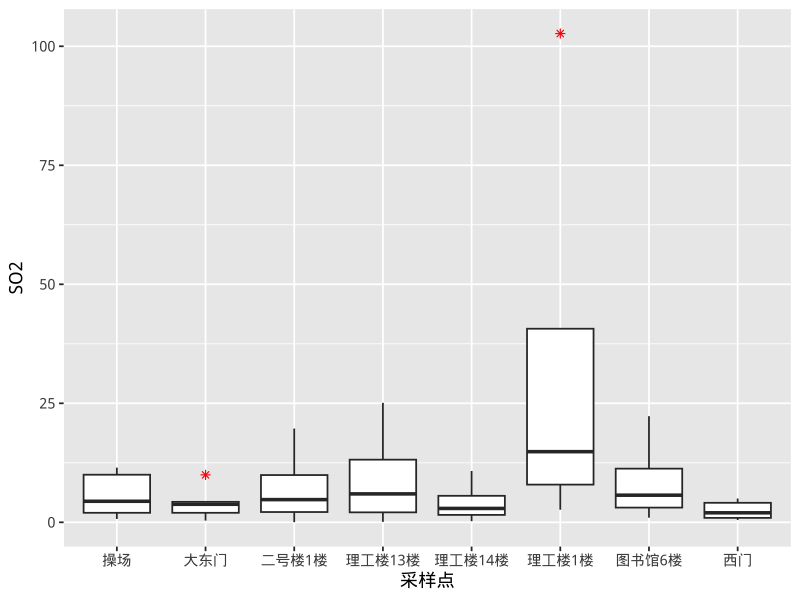
\includegraphics[width=\textwidth]{dataout/SO2_boxplot.png}
        \caption{SO$_2$浓度箱线图}
        \label{fig:SO2_boxplot}
    \end{subfigure}
    \hfill
    \begin{subfigure}[b]{0.32\textwidth}
        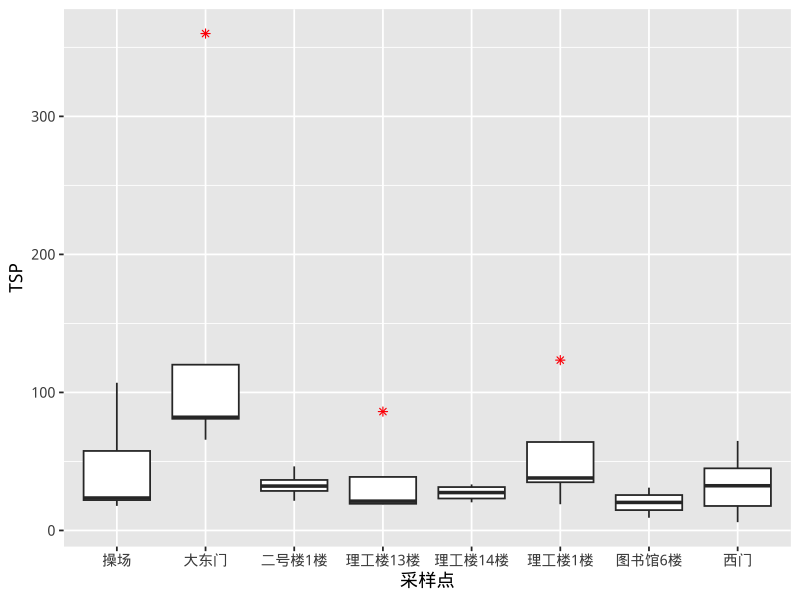
\includegraphics[width=\textwidth]{dataout/TSP_boxplot.png}
        \caption{TSP浓度箱线图}
        \label{fig:TSP_boxplot}
    \end{subfigure}
    \hfill
    \begin{subfigure}[b]{0.32\textwidth}
        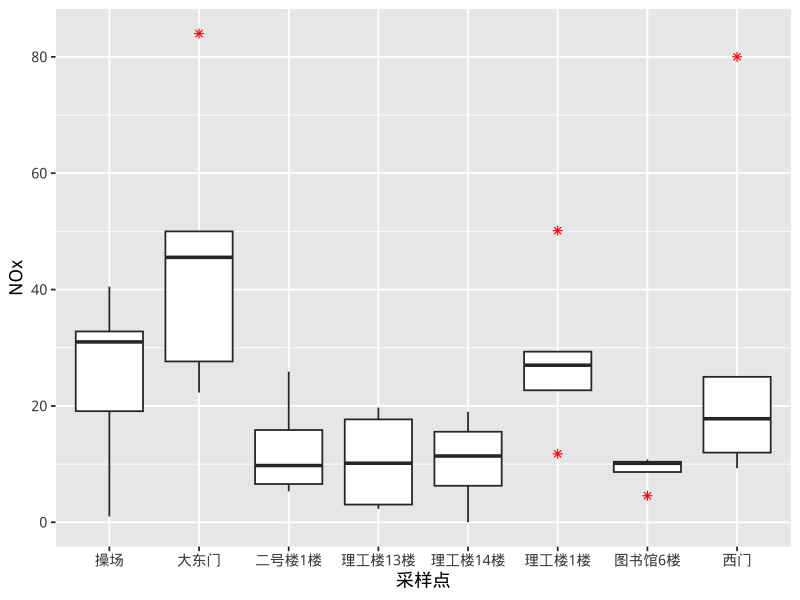
\includegraphics[width=\textwidth]{dataout/NOx_boxplot.png}
        \caption{NO$_x$浓度箱线图}
        \label{fig:NOx_boxplot}
    \end{subfigure}
    \caption{各监测点SO$_2$、TSP、NO$_x$浓度箱线图(a、b、c)}
    \label{fig:boxplots}
\end{figure}

\section{监测结果与讨论}
\subsection{监测数据以及质量分析}
数据集一共包含44个有效样本,剔除了缺失值以及离群值,清洗过后各点位的SO$_2$、NO$_x$和TSP浓度均值和标准差如表\ref{tab:pollutant_concentration}所示。

\begin{table}[htbp]
\centering
\caption{各个点位SO$_2$、NO$_x$和TSP浓度均值和标准差}
\label{tab:pollutant_concentration}
\begin{tabular}{cccccccc}
\hline
地点 & SO2均值 & SO2标准差 & NOx均值 & NOx标准差 & TSP均值 & TSP标准差 \\
\hline
二号楼1楼 & 7.32 & 8.69 & 12.7 & 9.33 & 33.1 & 10.3 \\
图书馆6楼 & 8.67 & 9.48 & 10.4 & 0.405 & 20.2 & 10.9 \\
大东门 & 2.61 & 1.79 & 36.4 & 13.5 & 87.2 & 23.2 \\
操场 & 5.72 & 4.80 & 24.9 & 15.4 & 45.6 & 37.9 \\
理工楼13楼 & 9.29 & 11.2 & 10.6 & 90.6 & 20.5 & 2.19 \\
理工楼14楼 & 4.21 & 4.62 & 10.5 & 8.20 & 27.1 & 5.97 \\
理工楼1楼 & 10.8 & 8.73 & 26.3 & 3.37 & 39.0 & 18.7 \\
西门 & 2.50 & 1.97 & 16.0 & 6.96 & 33.2 & 23.0 \\
\hline
\end{tabular}
\end{table}

\begin{figure}[htbp]
    \centering
    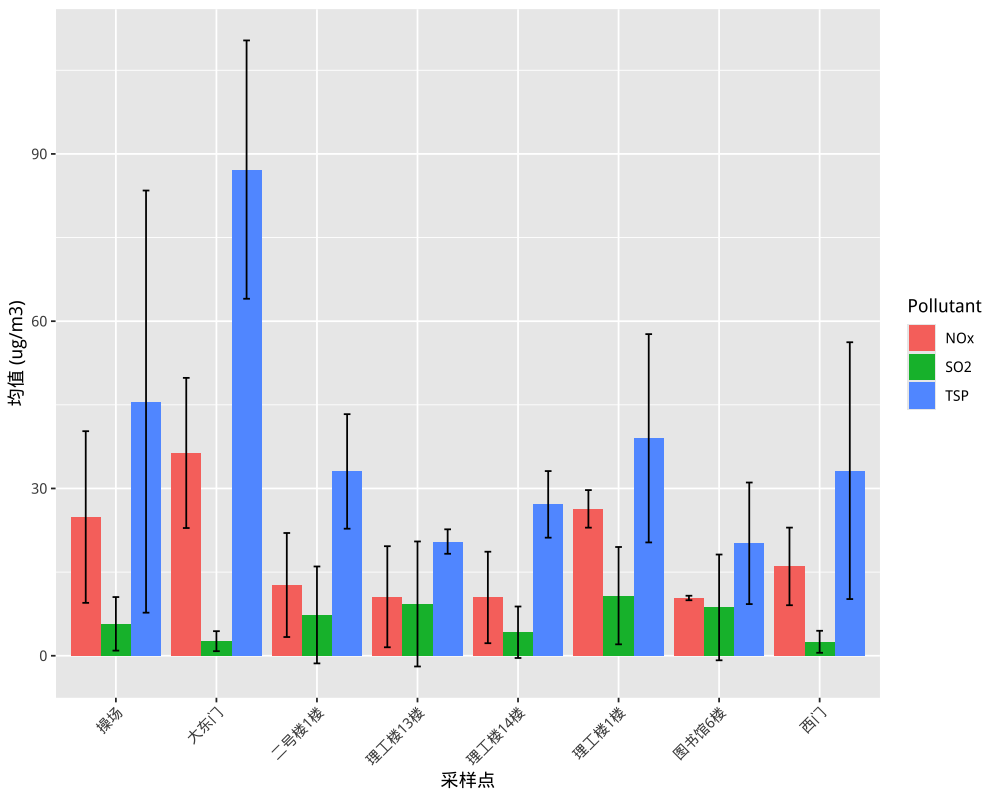
\includegraphics[width=0.8\textwidth]{dataout/site_mean_bar.png}
    \caption{各监测点SO$_2$、NO$_x$、TSP浓度均值柱状图}
    \label{fig:site_mean_bar}
\end{figure}

由图\ref{fig:boxplots}可以看出,本次监测实验的数据并不是很好,尤其是NO$_x$的标准差较大,说明各组实验操作不够规范,数据存在较大差异。SO$_2$和TSP的标准差相对较小,说明各组实验操作相对规范。

\subsection{时空分布规律分析}
\subsubsection{空间分布规律分析}
结合图\ref{fig:boxplots}可以看出,室内地点污染物浓度相对较低,可能是由于通风良好并且原理污染源,但是理工楼一楼采样点存在例外,可能是由于理工楼一楼靠近实验室,并且通风较差,导致污染物浓度较高。
观察室外点位发现,大东门和西门的污染物浓度较高,可能是由于靠近主干道,交通流量较大,导致污染物浓度较高。
操场点位数据波动性较大,推测应该是场地较为开阔,容易受外来污染物影响。

\begin{figure}[htbp]
    \centering
    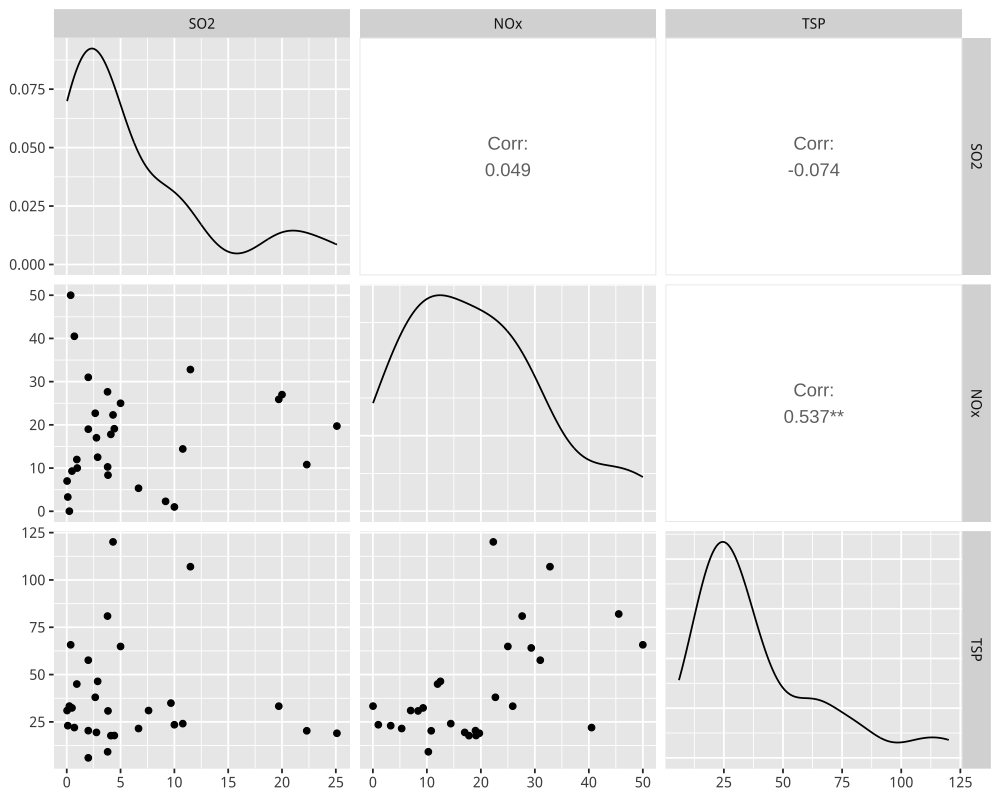
\includegraphics[width=0.7\textwidth]{dataout/cor_matrix.png}
    \caption{SO$_2$、NO$_x$、TSP浓度相关性矩阵热力图}
    \label{fig:cor_matrix}
\end{figure}

由图\ref{fig:cor_matrix}分析可以发现TSP与NO$_x$呈现中等强正相关(0.537),SO$_2$浓度与其他两者的相关性较弱。再分析各污染物浓度与监测地点的相关性,发现NO$_x$与TSP的浓度与地点相关性较强,t值分别为3.45和2.89,P值均小于0.05.



\subsubsection{时间分布规律分析}
由图\ref{fig:daily_mean_trend}可以看出,TSP浓度在5月17日出现峰值,查阅实验记录和当日天气状况发现当日有大风天气,导致TSP浓度升高(尤其是大东门)。
SO$_2$浓度较为稳定,NO$_x$的浓度存在升高的趋势。

\begin{figure}[htbp]
    \centering
    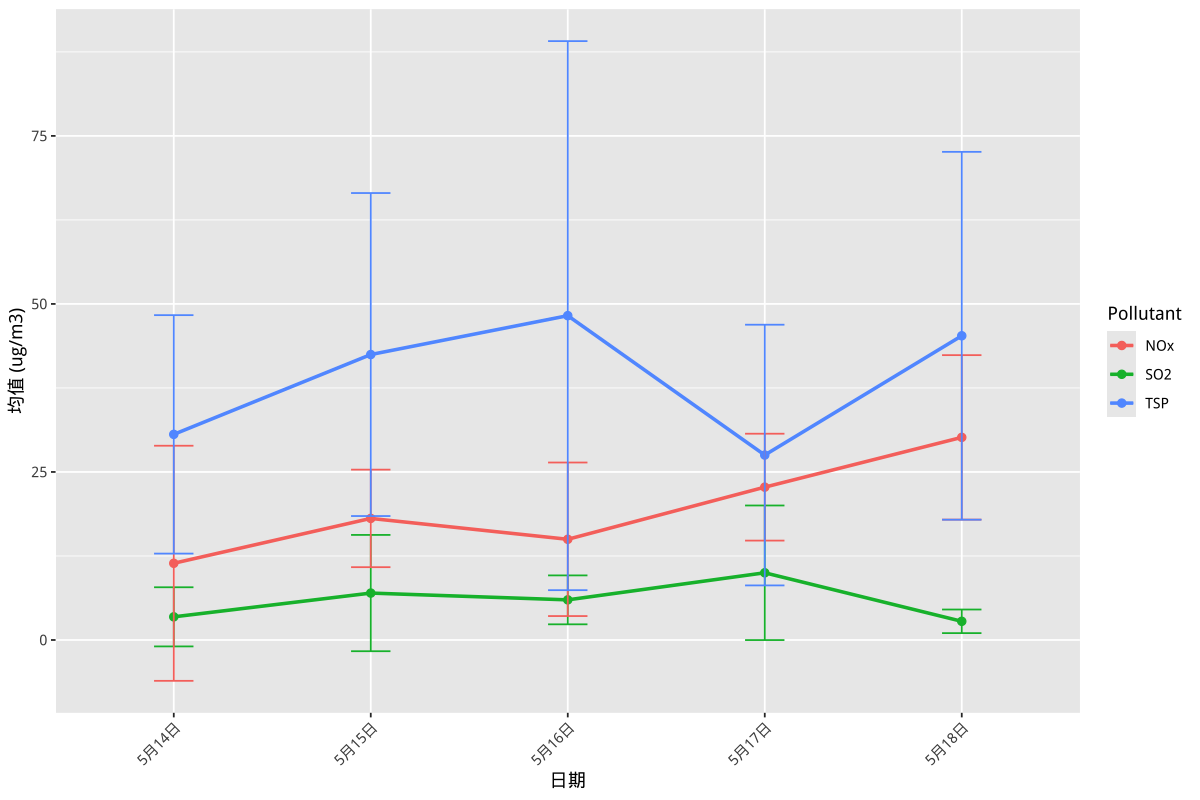
\includegraphics[width=0.8\textwidth]{dataout/daily_mean_trend.png}
    \caption{SO$_2$、NO$_x$、TSP日均浓度变化趋势}
    \label{fig:daily_mean_trend}
\end{figure}
\subsection{讨论与建议}
监测显示,TSP浓度偶尔超过中国环境空气质量标准(GB~3095--2012)每日限值$150\,\mu\mathrm{g}/\mathrm{m}^3$,特别是在大东门。t检验结果表明,NO$_x$和TSP浓度在大东门和西门显著较高,确认了交通排放和道路扬尘是主要污染源。SO$_2$水平较低且无显著区域差异,表明工业影响较小。

在分析实验数据时发现,各组之间的差异较大,尤其是NO$_x$,说明存在实验规范问题,以及所上交的数据单位各不相同,还有许多组在计算时出现错误,搞错数量级。建议在下次实验前应该先做好预习工作,实验测试时应该添加平行组,减少人为误差,提交实验数据时需要核对数据是否计算正确,以及统一数据单位。

\section{结论}

根据监测数据,中央民族大学海淀校区的空气质量总体处于可接受水平,但在某些时间和地点存在局部超标现象,尤其是在靠近交通要道的区域。以下是对各污染物浓度的具体评价:

二氧化硫(SO$_2$):SO$_2$浓度均值范围为3.34–27.00 $\mu$g/m$^3$,远低于GB~3095--2012一级标准(日均限值60 $\mu$g/m$^3$)。所有采样点的SO$_2$浓度均符合标准,表明校区未受到显著的工业或燃煤排放影响。t检验显示交通要道与非交通区域的SO$_2$浓度无显著差异($p=0.22$),进一步确认SO$_2$污染来源与交通活动无关。

氮氧化物(NO$_x$):NO$_x$浓度均值范围为8.28–45.90 $\mu$g/m$^3$,低于国家标准(日均限值80 $\mu$g/m$^3$)。然而,靠近交通要道的大东门显示较高浓度,t检验表明交通要道区域的NO$_x$浓度显著高于非交通区域($p=0.001$),反映了车辆尾气排放的明显影响。尽管未超标,交通密集区域的NO$_x$水平需关注。

总悬浮颗粒物(TSP):TSP浓度均值范围为20.17–141.75 $\mu$g/m$^3$,部分采样点(如大东门,5月16–17日单日值359.996 $\mu$g/m$^3$)超过GB~3095--2012一级标准(日均限值120 $\mu$g/m$^3$)。t检验显示交通要道区域的TSP浓度显著高于非交通区域($p=0.006$),表明道路扬尘和车辆活动是主要来源。TSP的局部超标是校区空气质量的主要问题。

综合来看,SO$_2$和NO$_x$浓度符合国家一级标准,空气质量良好;但TSP在特定时间和地点(尤其是大东门)存在超标现象,整体空气质量评级为良好但需局部改善。

\reference


\end{document}